\begin{align}
\vec{A}&=\myvec{0 \\ 0},\  
\Vec{B}=\myvec{36 \\ 15} \\ 
\implies 
\vec{d}&=\norm{\vec{A}-\vec{B}}
=39
\end{align}
See 
\figref{fig:10/7/1/2vec}.
\begin{figure}[H]
\centering
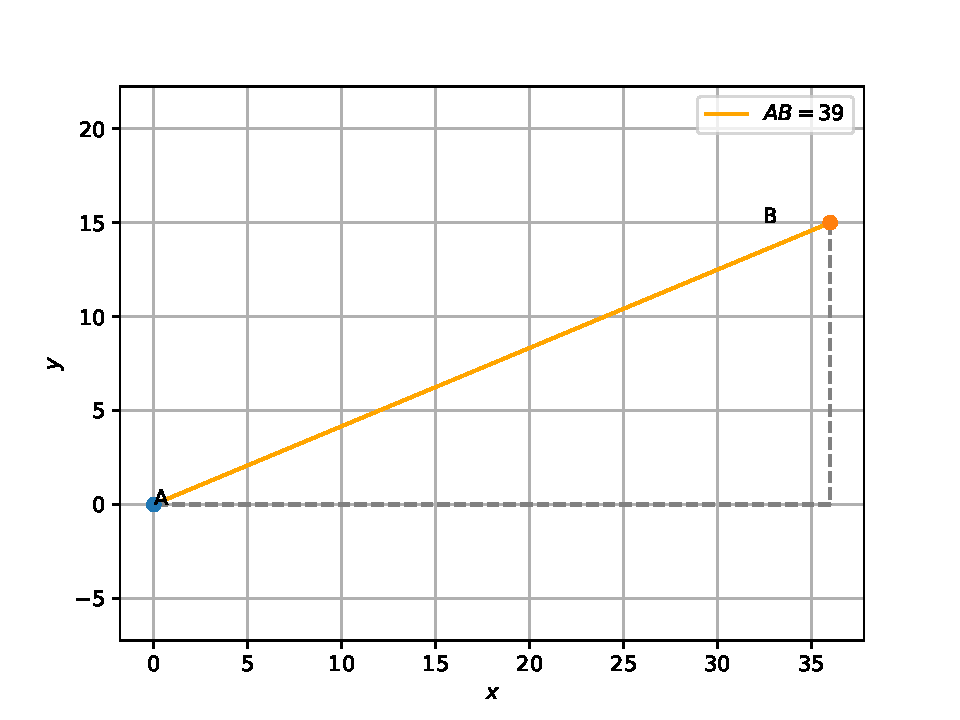
\includegraphics[width=0.75\columnwidth]{chapters/10/7/1/2/figs/vec.pdf}
\caption{}
\label{fig:10/7/1/2vec}
\end{figure}
